\subsection{Traditional cuts on the electron lab coordinates $\phi, \theta, p$}
The fiducial cut in the lab coordinates has been determined during the $\pi^0$ analysis in
the $\Delta(1232)$ region \cite{bib:pi0_Delta}.
For each sector, an empirical cut on $\phi$ is introduced as a function of theta and momentum:
$$
\phi \,\,\le\,\, \Delta\phi \,(\theta, p)
$$
which is aimed to define regions of phase space whose distributions are flat in $\phi$.
After careful studies, and following a common approach between different CLAS experiments, the mathematical
form of the cut depends on 6 parameters  $C_i$
and assumes the form:\vspace{-0.3 cm}
$$
\begin{array}{c c c}
    \\
    \Delta\phi   & = & C_4 \left( \sin (\theta - \theta_{cut}) \right) ^{\,E} \\
    \\
    E        & = & C_3\, p\, ^{C_5} \\
    \\
    \theta_{cut} & = & C_1 + \frac{C_2}{p + C_6}
\end{array}
$$

The $\phi$ vs $\theta$ distribution were divided in 10 different momentum bins from $1.6$ to $4.6$ GeV.
Fig.~\ref{fig:fidu_etph} shows one example ($p=1.9-2.2$ GeV) of such distributions.
The $\phi$ distributions are also plotted for $\theta$ slices one degree wide as in Fig.~\ref{fig:fidu_ephis}
and the $C_i$ parameters are adjusted empirically.

Table \ref{tab:fid_epars} shows the 6 parameters obtained. Fig.~\ref{fig:fidu_e3d} shows
the fiducial cut as a function of $p$, $\theta$ and $\phi$ for sector 1.

\begin{table}[h]
    \begin{center}
        \begin{tabular}{|c|c|c|c|c|c|c|}
            \hline
            Sector & $C_1$ & $C_2$ & $C_3$ & $C_4$ & $C_5$    & $C_6$ \\
            \hline
            1      & 12.0  & 20.0  & 0.32  & 32.0  & 0.416667 & 0.14  \\
            2      & //    & 20.7  & 0.36  & 34.0  & //       & //    \\
            3      & //    & 20.2  & 0.32  & 32.0  & //       & //    \\
            4      & //    & 20.5  & 0.32  & 32.0  & //       & //    \\
            5      & //    & 20.5  & 0.29  & 32.0  & //       & //    \\
            6      & //    & 20.0  & 0.32  & 32.0  & //       & //    \\
            \hline
        \end{tabular}
    \end{center}
    \caption[The 6 parameters for electron fiducial cut for each of the 6 sectors.]
    { The 6 parameters for electron fiducial cut for each of the 6 sectors.
    Only $C_2$, $C_3$, $C_4$ are sector dependent. }
    \label{tab:fid_epars}
\end{table}


\begin{figure}[h]
    \centering
    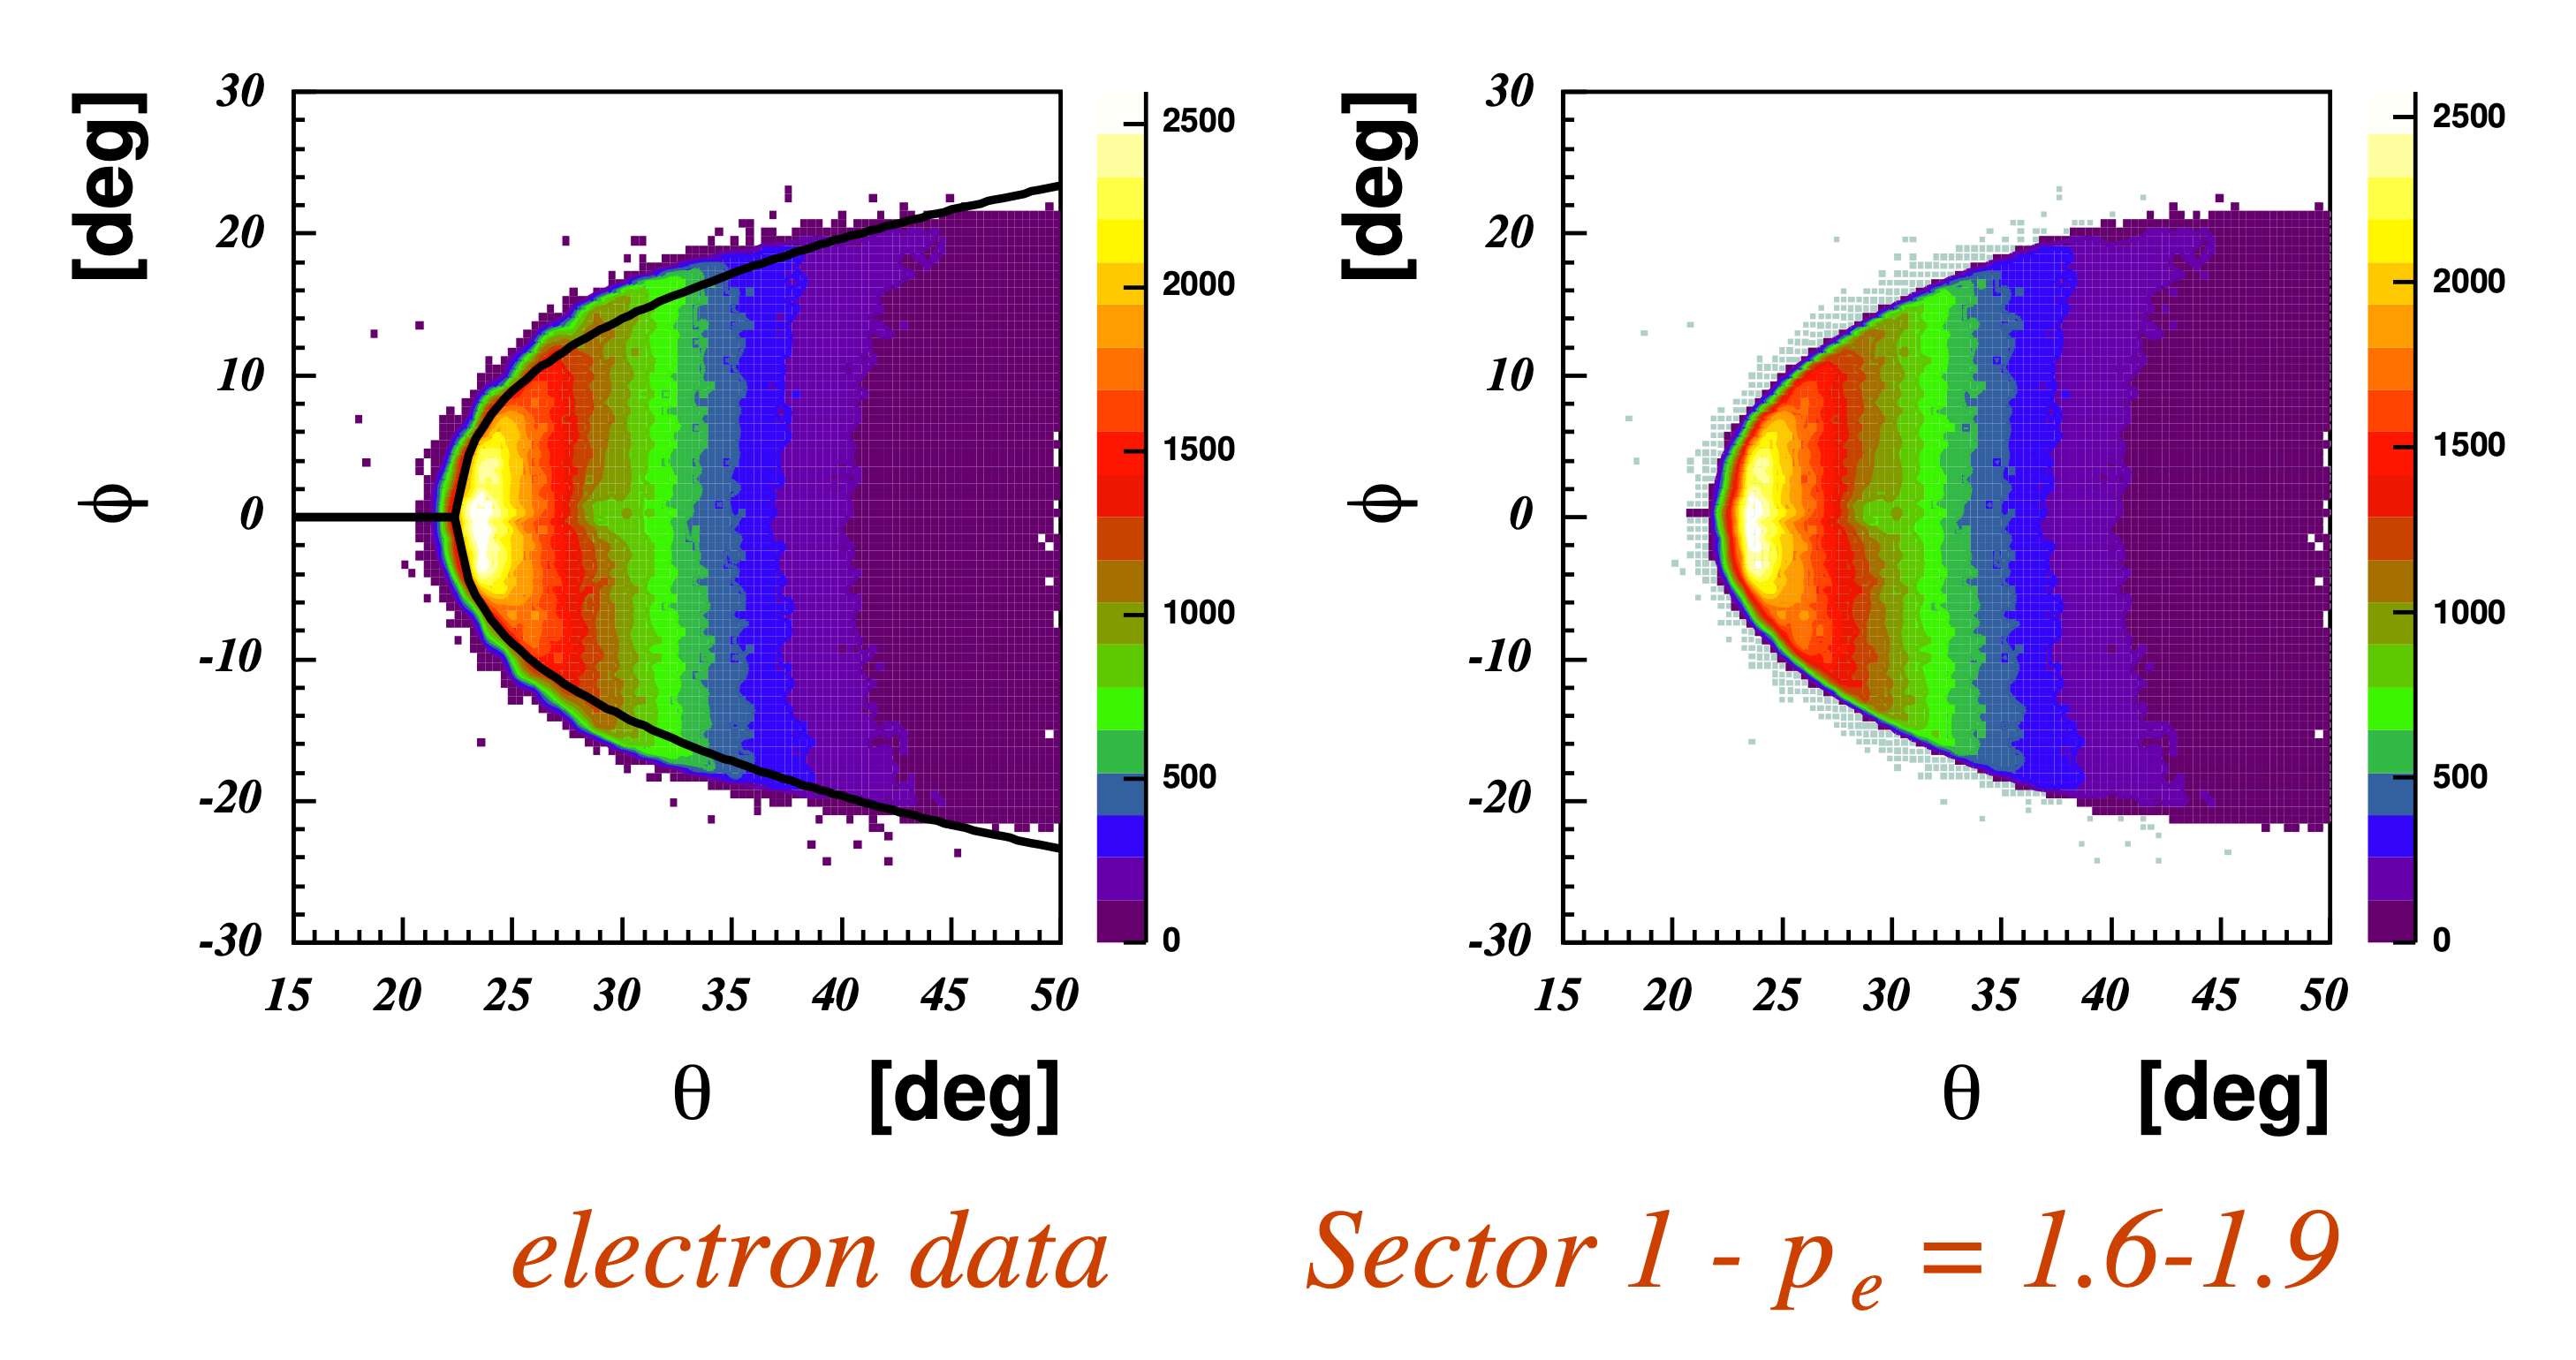
\includegraphics[width=0.9\textwidth ]{img/electron_tph}
    \caption{$\phi$ versus $\theta$ for sector 1 and $p=1.6-1.9$ GeV after the
    electron ID. Left: before fiducial cut. Right: before fiducial cut
        (box/gray) and after fiducial cut (color contour). }
    \label{fig:fidu_etph}
\end{figure}

\begin{figure}[h]
    \centering
    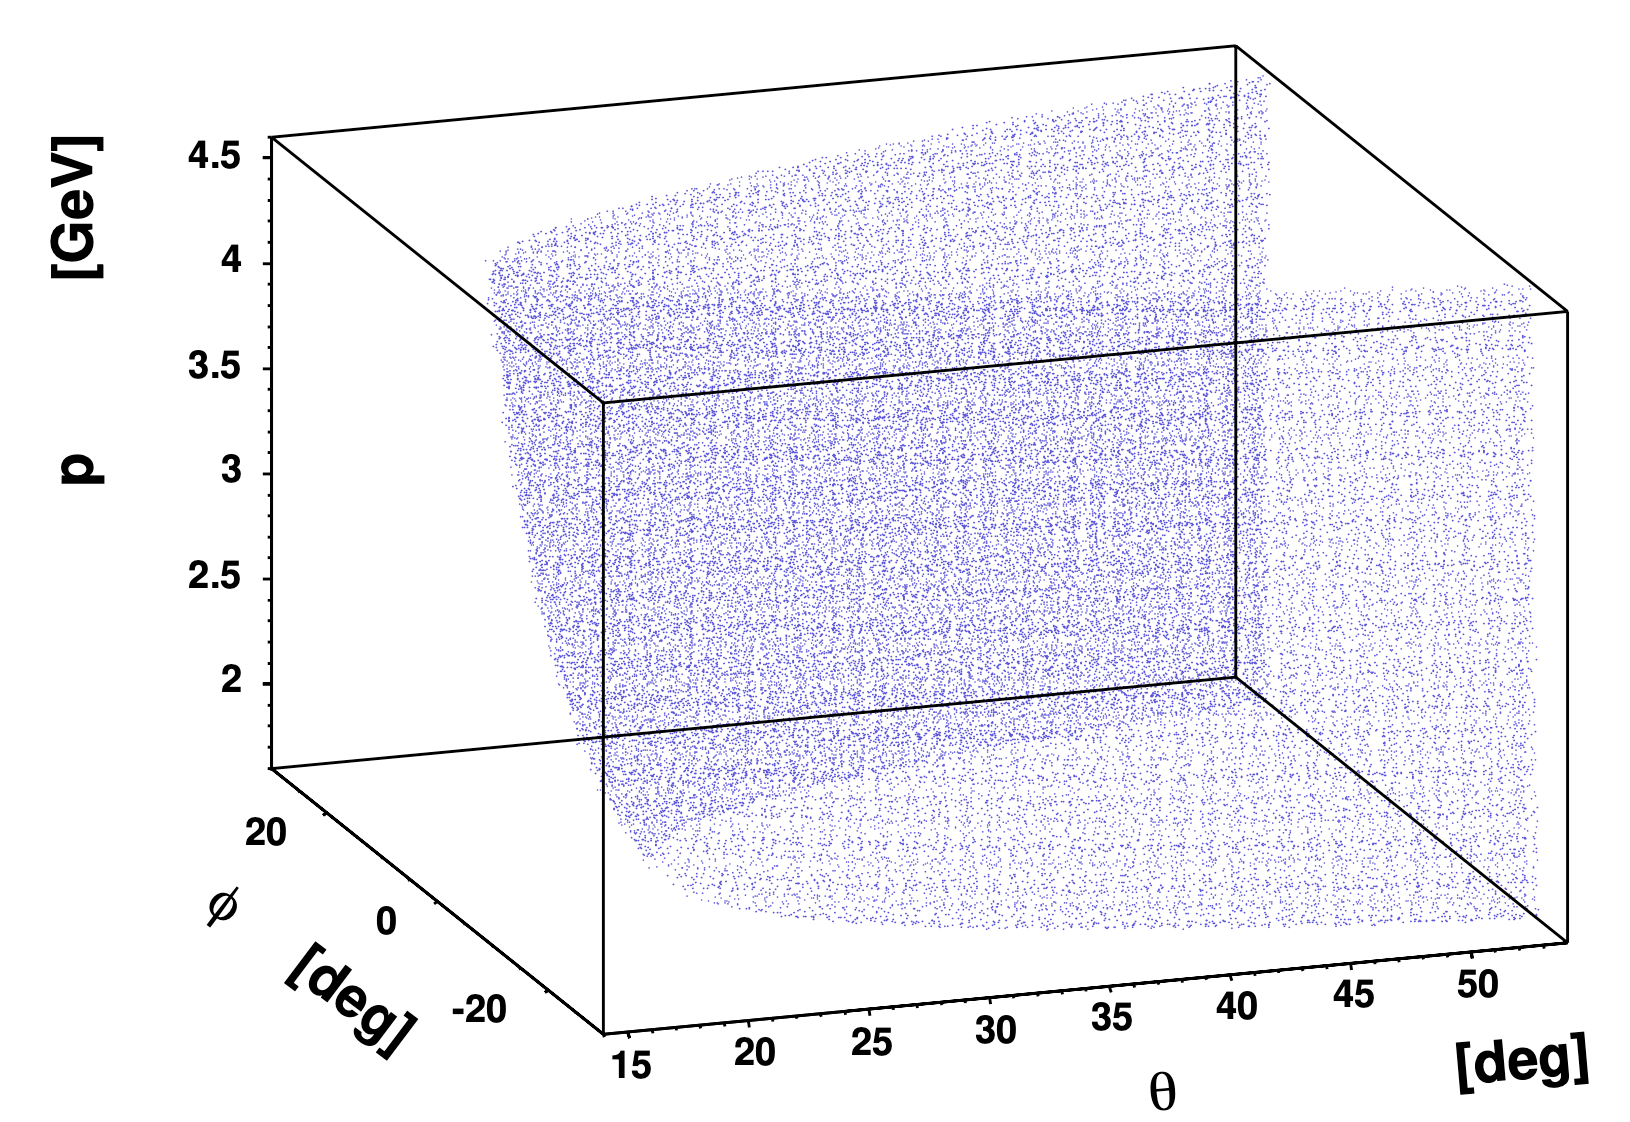
\includegraphics[width=0.9\textwidth ]{img/electron_tphp}
    \caption{The electron fiducial cut for sector 1 as a function of  $\phi, \theta, p$.
    The cut starting point moves back
    as the momentum increases (and $\theta$ decreases). This causes the cut
    to narrow up with momemtum because electrons are detected near the lower
    edges of the detectors.}
    \label{fig:fidu_e3d}
\end{figure}



\clearpage\newpage


\begin{figure}[ht]
    \centering
    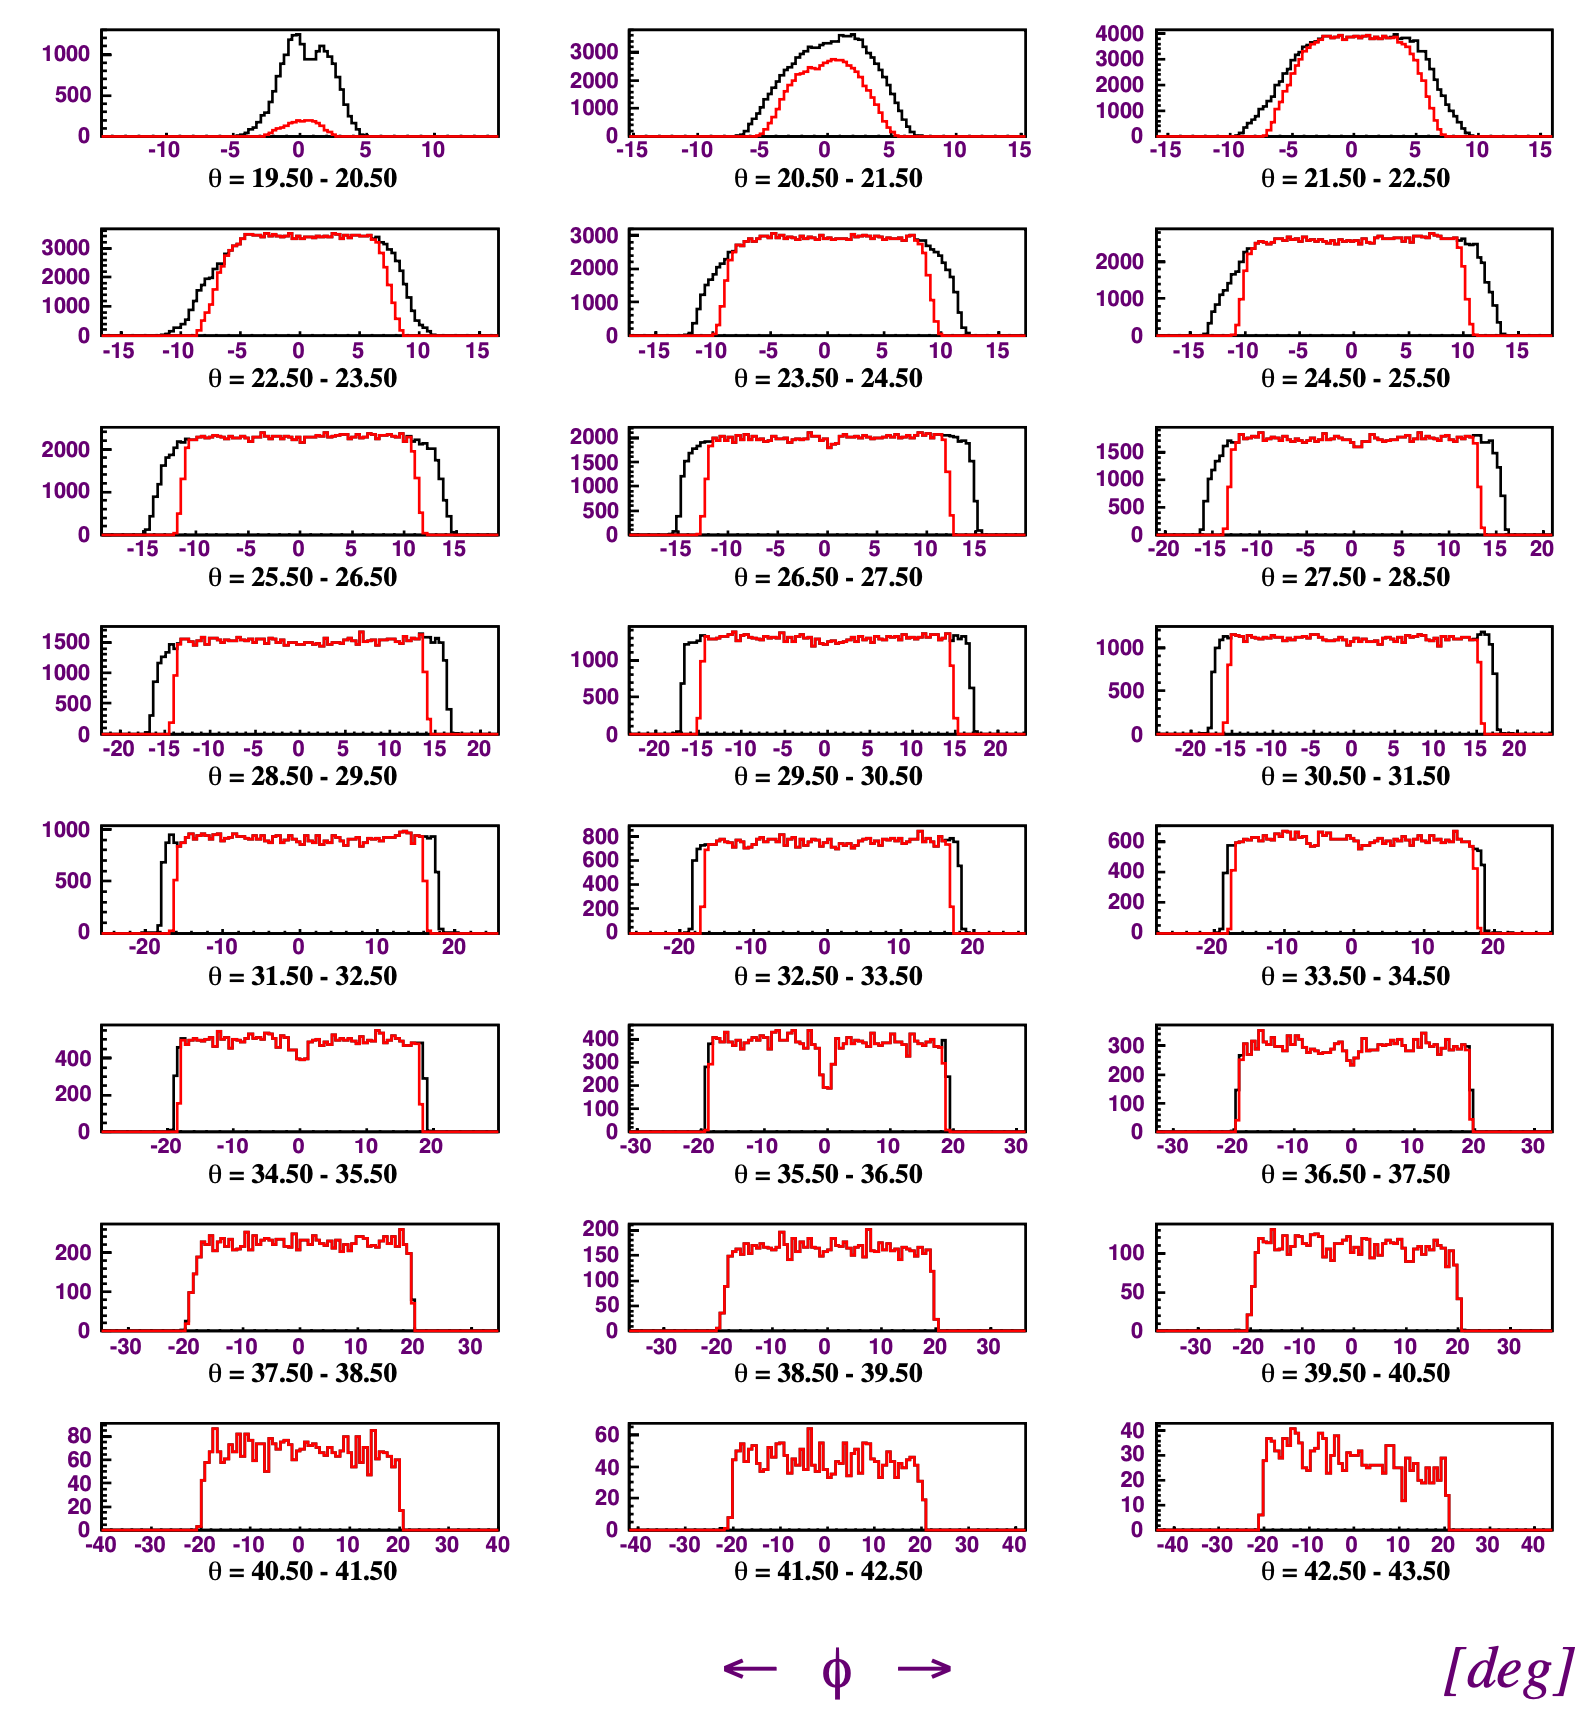
\includegraphics[width=0.98\textwidth ]{img/electron_phis}
    \caption{$\phi$ distributions (sector 3) for different $\theta$ and
        $p=1.9-2.2$ GeV. Black: before fiducial cut. Red: after fiducial cut.
        \v Cerenkov inefficiency (section \ref{sec:cc_eff}) is responsible
        for some irregularities at $\phi = 0$ (for example at
        $\theta = 35.5^0 - 36.5^0$) while drift chambers and time of flight
        inefficiency (section \ref{sec:dc_ineff}) causes other irregularities
        (for example at  $\theta = 42.5^0 - 43.5^0$).}
    \label{fig:fidu_ephis}
\end{figure}


\clearpage\newpage




\subsection{ $\theta$ versus momentum cuts}
Sector 2, 5 and 6 present holes and depletions (mainly because of dead time of flight paddles)
which were taken care of with the
cuts in the $\theta$ vs $p$ plane. An example of such cut is shown in Fig.~\ref{fig:fidu_etp5}.

\begin{figure}[h]
 \begin{center}
 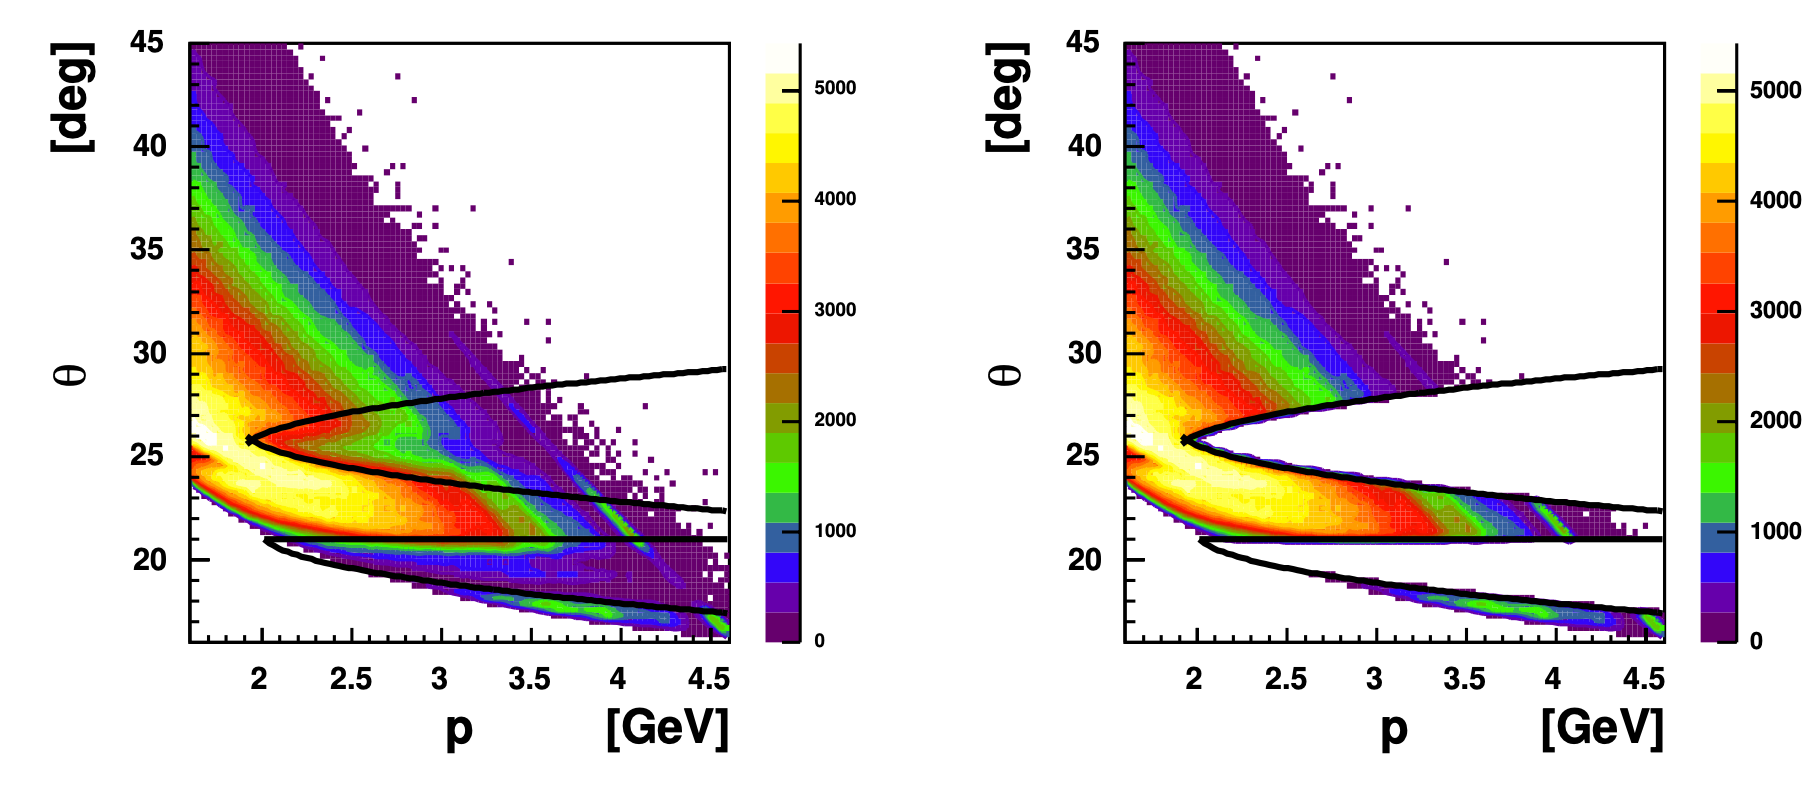
\includegraphics[width=0.98\textwidth ]{img/electron_tp5}
  \caption[ $\theta$ versus $p$ for sector 5]
          { $\theta$ versus $p$ for sector 5. Two depletions are clearly visible and cut out.}
 \label{fig:fidu_etp5}
 \end{center}
\end{figure}


